\documentclass[10pt,journal,compsoc]{IEEEtran}
\usepackage[utf8]{inputenc}

%Language
\usepackage[english]{babel}

% Citation
\usepackage[nocompress]{cite}

% Graphics
\usepackage[pdftex]{graphicx}
\graphicspath{{.shared/img/}{./individual/img/}}
\DeclareGraphicsExtensions{.pdf,.jpeg,.png}

% Math
\usepackage{mathtools}
\usepackage{amsmath}
\usepackage{amsfonts}
\usepackage{amssymb}
\interdisplaylinepenalty=2500

%Lay out
\usepackage{xspace}
\usepackage{booktabs}

%Pseudo Code
\usepackage{algpseudocode}

% Floats
\usepackage[caption=false,font=footnotesize,labelfont=sf,textfont=sf]{subfig}
\usepackage{stfloats}

%Hyperlinks
\usepackage{url}
\usepackage{varioref}
\usepackage{hyperref}
\usepackage[noabbrev, capitalise, nameinlink]{cleveref}
\usepackage{etoolbox}
% Patch cleverref for use with ieee, source: http://tex.stackexchange.com/a/250739
\makeatletter
\patchcmd{\@IEEEyesnumber}
  {\stepcounter}
  {\refstepcounter}
  {}{}
\patchcmd{\@@IEEEeqnarray}
  {\stepcounter}
  {\refstepcounter}
  {}{}
\patchcmd{\@@IEEEeqnarraycr}
  {\stepcounter{IEEEsubequation}}
  {\refstepcounter{IEEEsubequation}}
  {}{}
\patchcmd{\@@IEEEeqnarraycr}
  {\stepcounter{IEEEsubequation}}
  {\refstepcounter{IEEEsubequation}}
  {}{}
\patchcmd{\@@IEEEeqnarraycr}
  {\stepcounter{IEEEequation}}
  {\refstepcounter{IEEEequation}}
  {}{}
\patchcmd{\@@IEEEeqnarraycr}
  {\stepcounter{IEEEequation}}
  {\refstepcounter{IEEEequation}}
  {}{}
\makeatother

%Lists
\usepackage[inline]{enumitem}
\crefname{enumi}{stage}{stages}  
\Crefname{enumi}{Stage}{Stages}

%Math
\DeclarePairedDelimiter\abs{\lvert}{\rvert}%
\DeclarePairedDelimiter\norm{\lVert}{\rVert}
\makeatletter
\let\oldabs\abs
\def\abs{\@ifstar{\oldabs}{\oldabs*}}
\let\oldnorm\norm
\def\norm{\@ifstar{\oldnorm}{\oldnorm*}}
\makeatother

%Custom commands
\newcommand{\bigOh}[1]{\ensuremath{\mathcal{O}\left(#1\right)}}
\renewcommand{\t}[1]{\ensuremath{\mathit{#1}}}
\newcommand{\function}[2]{\textsc{#1}(#2)}

%Shortcuts
\newcommand{\astar}{A*\xspace}
\newcommand{\knnk}{\ensuremath{\mathcal{K}}\xspace}
\newcommand{\knn}{\knnk-NN\xspace}
\newcommand{\Knn}{\knnk-nearest neighbor\xspace}

%Temporary
\usepackage{layouts}
\usepackage[obeyFinal]{todonotes}
\newcommand{\angelo}[1]{\todo[color=blue!20, inline]{\textbf{Angelo: }#1}}
\newcommand{\laura}[1]{\todo[color=green!20, inline]{\textbf{Laura: }#1}}
\newcommand{\timemachine}[1]{\todo[color=red!20, inline]{\textbf{Given a time machine: }#1}}

\begin{document}

%!TEX root = /Users/laura/Repositories/HandwritingRecognition/report/main.tex
\title{Recognizing 12th Century Handwriting in the Roman Alphabet with Binary Over Segmentation}
\author{L.E.N. Baakman (S1869140)}

\markboth{Handwriting Recognition,~2015-2016}%
{Baakman: Recognizing 12th Century Handwriting in the Roman Alphabet with Binary Over Segmentation}

%!TEX root = /Users/laura/Repositories/HandwritingRecognition/report/main.tex
\IEEEtitleabstractindextext{%
\begin{abstract}
	% \todo[inline]{Motivation: Why do we care about the problem and the results? If the problem isn't obviously ``interesting" it might be better to put motivation first; but if your work is incremental progress on a problem that is widely recognized as important, then it is probably better to put the problem statement first to indicate which piece of the larger problem you are breaking off to work on. This section should include the importance of your work, the difficulty of the area, and the impact it might have if successful.}
	One of the most difficult steps in the process of off-line handwriting recognition is the segmentation of characters. 
	% \todo[inline]{Problem Statement: What problem are you trying to solve? What is the scope of your work (a generalized approach, or for a specific situation)? Be careful not to use too much jargon. In some cases it is appropriate to put the problem statement before the motivation, but usually this only works if most readers already understand why the problem is important.}
	This paper introduces a binary over segmentation approach that aims to reduce chain failure without being computationally expensive.
	% \todo[inline]{Approach: How did you go about solving or making progress on the problem? Did you use simulation, analytic models, prototype construction, or analysis of field data for an actual product? What was the extent of your work (did you look at one application program or a hundred programs in twenty different programming languages?) What important variables did you control, ignore, or measure?}
	This is done by starting segmentation in the middle of the image instead of moving from left to right. Images of characters are not validated by the use of the recognizer but based on the properties of the image, such as its dimensions. 
	% \todo[inline]{Results: What's the answer? Specifically, most good computer architecture papers conclude that something is so many percent faster, cheaper, smaller, or otherwise better than something else. Put the result there, in numbers. Avoid vague, hand-waving results such as ``very", ``small", or ``significant." If you must be vague, you are only given license to do so when you can talk about orders-of-magnitude improvement. There is a tension here in that you should not provide numbers that can be easily misinterpreted, but on the other hand you don't have room for all the caveats.}
	The method has been tested on two 12th century texts, and the results of the segmentation seem promising. 
	% \todo[inline]{Conclusions: What are the implications of your answer? Is it going to change the world (unlikely), be a significant ``win", be a nice hack, or simply serve as a road sign indicating that this path is a waste of time (all of the previous results are useful). Are your results general, potentially generalizable, or specific to a particular case?}
\end{abstract}

% Note that keywords are not normally used for peerreview papers.
\begin{IEEEkeywords}
Handwriting recognition, Segmentation algorithm, OCR, Pattern Recognition.
\end{IEEEkeywords}}

\maketitle

\IEEEdisplaynontitleabstractindextext
\IEEEpeerreviewmaketitle

\IEEEraisesectionheading{\section{Introduction}\label{s:introduction}}
%!TEX root = ../main.tex

In section \ref{ss:methods:preprocessing} we present the process of cleaning our textual data. In section \ref{ss:methods:characterSegmentation} we show how we split the words into characters whilst in section \ref{ss:methods:featureExtraction} we show the features we extracted from the characters to be used in the classification process. In section \ref{ss:methods:machineLearing} we present our machine learning approach and in section \ref{s:results} we present our results for both the characters and the words. Finally in section \ref{s:discussion} and \ref{s:conclusion} we present the discussion as well as our conclusions respectively.

\section{Methods}
\label{s:methods}
%!TEX root = ../main.tex
In this section we discuss the inner workings of our recognizer. \Cref{ss:methods:preprocessing} shortly discusses how we preprocessed our images. The next section explains how given an external segmentation we extract the character images. \Cref{ss:methods:featureExtraction} presents the method we used to represent these images as feature vectors. The classification of this representation is discussed in \cref{ss:methods:recognition}. Finally the method used for post processing is introduced in \cref{ss:methods:postprocessing}.

\subsection{Preprocessing}
\label{ss:methods:preprocessing}
%!TEX root = ../../main.tex
For the handwriting to be effective we had to bring the data into a clean state. To this end we used a pipeline which is described below in figure \ref{fig:pipeline}. 

\begin{figure}[ht]
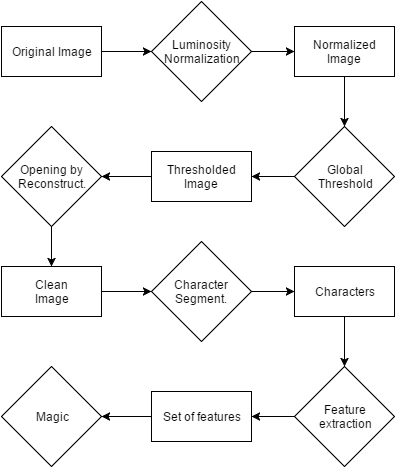
\includegraphics[width=8cm]{shared/img/pipeline.png}
\caption{Overview of our pipeline.}
\label{fig:pipeline}
\end{figure}

As the figure explains the first step is to normalize the luminosity of the image. This step is essential for the thresholding to work since in some parts of dataset the ink has worn off the pages. \Cref{fig:methods:preprocessing:lumNormalization} gives an example why luminosity normalization was necessary. In the above mentioned figure, we applied the same threshold filter with and without luminosity normalization and the results speak for themselves. By normalizing the luminosity we eliminate the need to adjust threshold values in later steps.

\begin{figure}
	\centering
	\subfloat[]{
		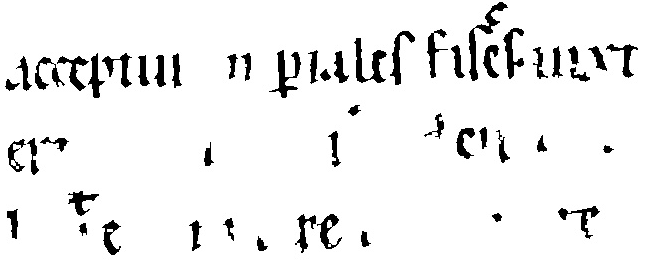
\includegraphics[width=\columnwidth]{shared/img/before_lum.png}%
		\label{fig:methods:preprocessing:lumNormalization:before}%
	}
	\hfil
	\subfloat[]{
		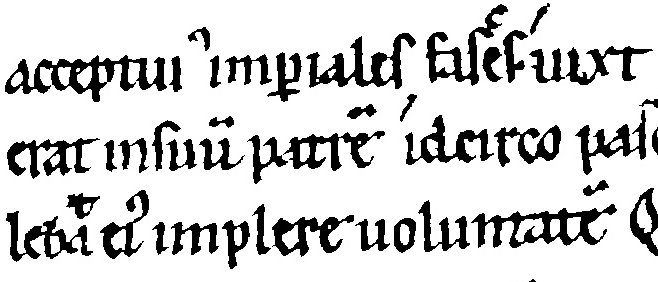
\includegraphics[width=\columnwidth]{shared/img/after_lum.png}%
		\label{fig:methods:preprocessing:lumNormalization:after}%
	}
	\caption{An image of text \protect\subref{fig:methods:preprocessing:lumNormalization:before} before and \protect\subref{fig:methods:preprocessing:lumNormalization:after} after luminization normalization.}
	\label{fig:methods:preprocessing:lumNormalization}
\end{figure}

The next step is to binarize the image and extract the clean text from it. For the binarization we tested the Otsu approach and global threshold and we settled with the first as it gave better results. To eliminate the what is left from the noise we applied opening by reconstruction. This has a result to miss some punctuation characters which however did not prove crucial to our learning process. %In figure \ref{} we can see the final result of the preprocessing of the data. 

\subsection{Internal Segmentation}
\label{ss:methods:characterSegmentation}
%!TEX root = ../../main.tex
\newcommand{\body}{\ensuremath{\t{body}}\xspace}
\newcommand{\strokewidth}{\ensuremath{\t{stroke\_w}}\xspace}
\newcommand{\segmentationpoints}{\ensuremath{\t{sps}}\xspace}
\newcommand{\segmentationpoint}{\ensuremath{\t{sp}}\xspace}
\newcommand{\image}{\ensuremath{\t{image}}\xspace}
\newcommand{\subimage}{\ensuremath{\t{sub\_image}}\xspace}
\newcommand{\leftsubimage}{\ensuremath{\t{left}}\xspace}
\newcommand{\rightsubimage}{\ensuremath{\t{right}}\xspace}
\newcommand{\segmentfurther}{\ensuremath{\t{todo}}\xspace}
\newcommand{\characters}{\ensuremath{\t{done}}\xspace}
\newcommand{\parameters}{\ensuremath{\t{parameters}}\xspace}

\begin{figure}[t]
	%!TEX root = ../../main.tex
\MakeRobust{\Call}

\begin{algorithmic}[0]
\Function{segment}{$\image,\, \parameters$}
\label{alg:line:bodyregion} \State \body $\gets$ \Call{body\_region}{\image}
\label{alg:line:strokewidth} \State \strokewidth $\gets$ \Call{stroke\_width}{\image} 
\item[]
\label{alg:line:segmentationpoints} \State \segmentationpoints $\gets$ \Call{segmentation\_points}{\body, \strokewidth} 
\State \segmentfurther, \characters $\gets$ [\image], []
\item[]
\label{alg:line:whileCondition} \While{\Call{continue}{~}}
	\label{alg:line:selectSubImage}\State $\subimage \gets$ \Call{select\_sub\_image}{\segmentfurther} 
	\label{alg:line:selectSegmentationPoint}\State $\segmentationpoint \gets$ \Call{select\_sp}{\segmentationpoints} 
	\label{alg:line:split}\State \leftsubimage, \rightsubimage $\gets$ \Call{split}{\subimage, \segmentationpoint}
	%
	\State \Call{add\_to\_correct\_list}{\leftsubimage, \characters, \segmentfurther}
	\State \Call{add\_to\_correct\_list}{\rightsubimage, \characters, \segmentfurther}
\EndWhile
\label{alg:line:merge}\State \textbf{return} \Call{merge}{\segmentfurther, \characters}
\EndFunction
\end{algorithmic}
	\caption{The Binary Over Segmentation Algorithm.}
	\label{alg:method:segmentation:algorithm}
\end{figure}

We use a form of binary over segmentation to recognize characters in the word, see \cref{alg:method:segmentation:algorithm}. This algorithm aims to segment an image on the most likely segmentation point. If these sub images are not characters they can be selected again for further segmentation. This segmenting of sub images is repeated until the termination condition has been reached. The final list of characters is the list of characters, \characters, merged with the list of images that could be segmented further, \segmentfurther. This merge also ensures that the order of the images is correct.

The \parameters passed to \function{segment}{} in \cref{alg:method:segmentation:algorithm} contain the maximum word length and the minimum, mean and maximum image width, height and number of foreground pixels. Other than maximum word length, these parameters are computed based on the train data, by collecting these data from each character image, the minimum, mean and maximum are computed over all measurements that fall within two standard deviations of the mean. The maximum word length is simply the length of the longest word in the train data.

The different functions used in \cref{alg:method:segmentation:algorithm} are discussed in \crefrange{sss:method:segmentaton:bodyregion}{sss:method:segmentaton:termination}.

\subsubsection{Body Region}
\label{sss:method:segmentaton:bodyregion}
	The body region is the part of the image between the lower and upper base line. The lower base line is computed as the mode of the minimum row index with a foreground pixel in each column. The upper baseline is computed similarly, but uses the maximum row index.

	Using the body region for the computation of the segmentation points reduces the influence of extensive ligatures \cite{lee2012binary}. \Cref{fig:method:segmentation:baseline} presents some examples of computed baselines. The first example, \Cref{fig:method:segmentation:baseline:succes}, reflects the intended outcome. The second example, \cref{fig:method:segmentation:baseline:failure}, draws the upper baseline too high, probably due too the extra curve on the last letter.

\subsubsection{Stroke Width}
\label{sss:method:segmentaton:strokwidth}
	The stroke width refers to how thick the stroke of a pen is. It is computed as the mode of the number of sequential foreground pixels in one row or column of pixels. As different pens or authors can write on the same page it is more robust to compute the stroke width per word image instead of per page image.

\subsubsection{Segmentation Points}
\label{sss:method:segmentaton:segmentationpoints}
	To find the segmentation lines we first determine the suspicious regions. A suspicious region is a region in the body of the word image where the vertical pixel density is greater than some threshold, $2 \cdot \strokewidth$. \Cref{fig:method:segmentation:suspiciousRegions} illustrates the suspicious regions found in a word. 

	\begin{figure}
		\centering
		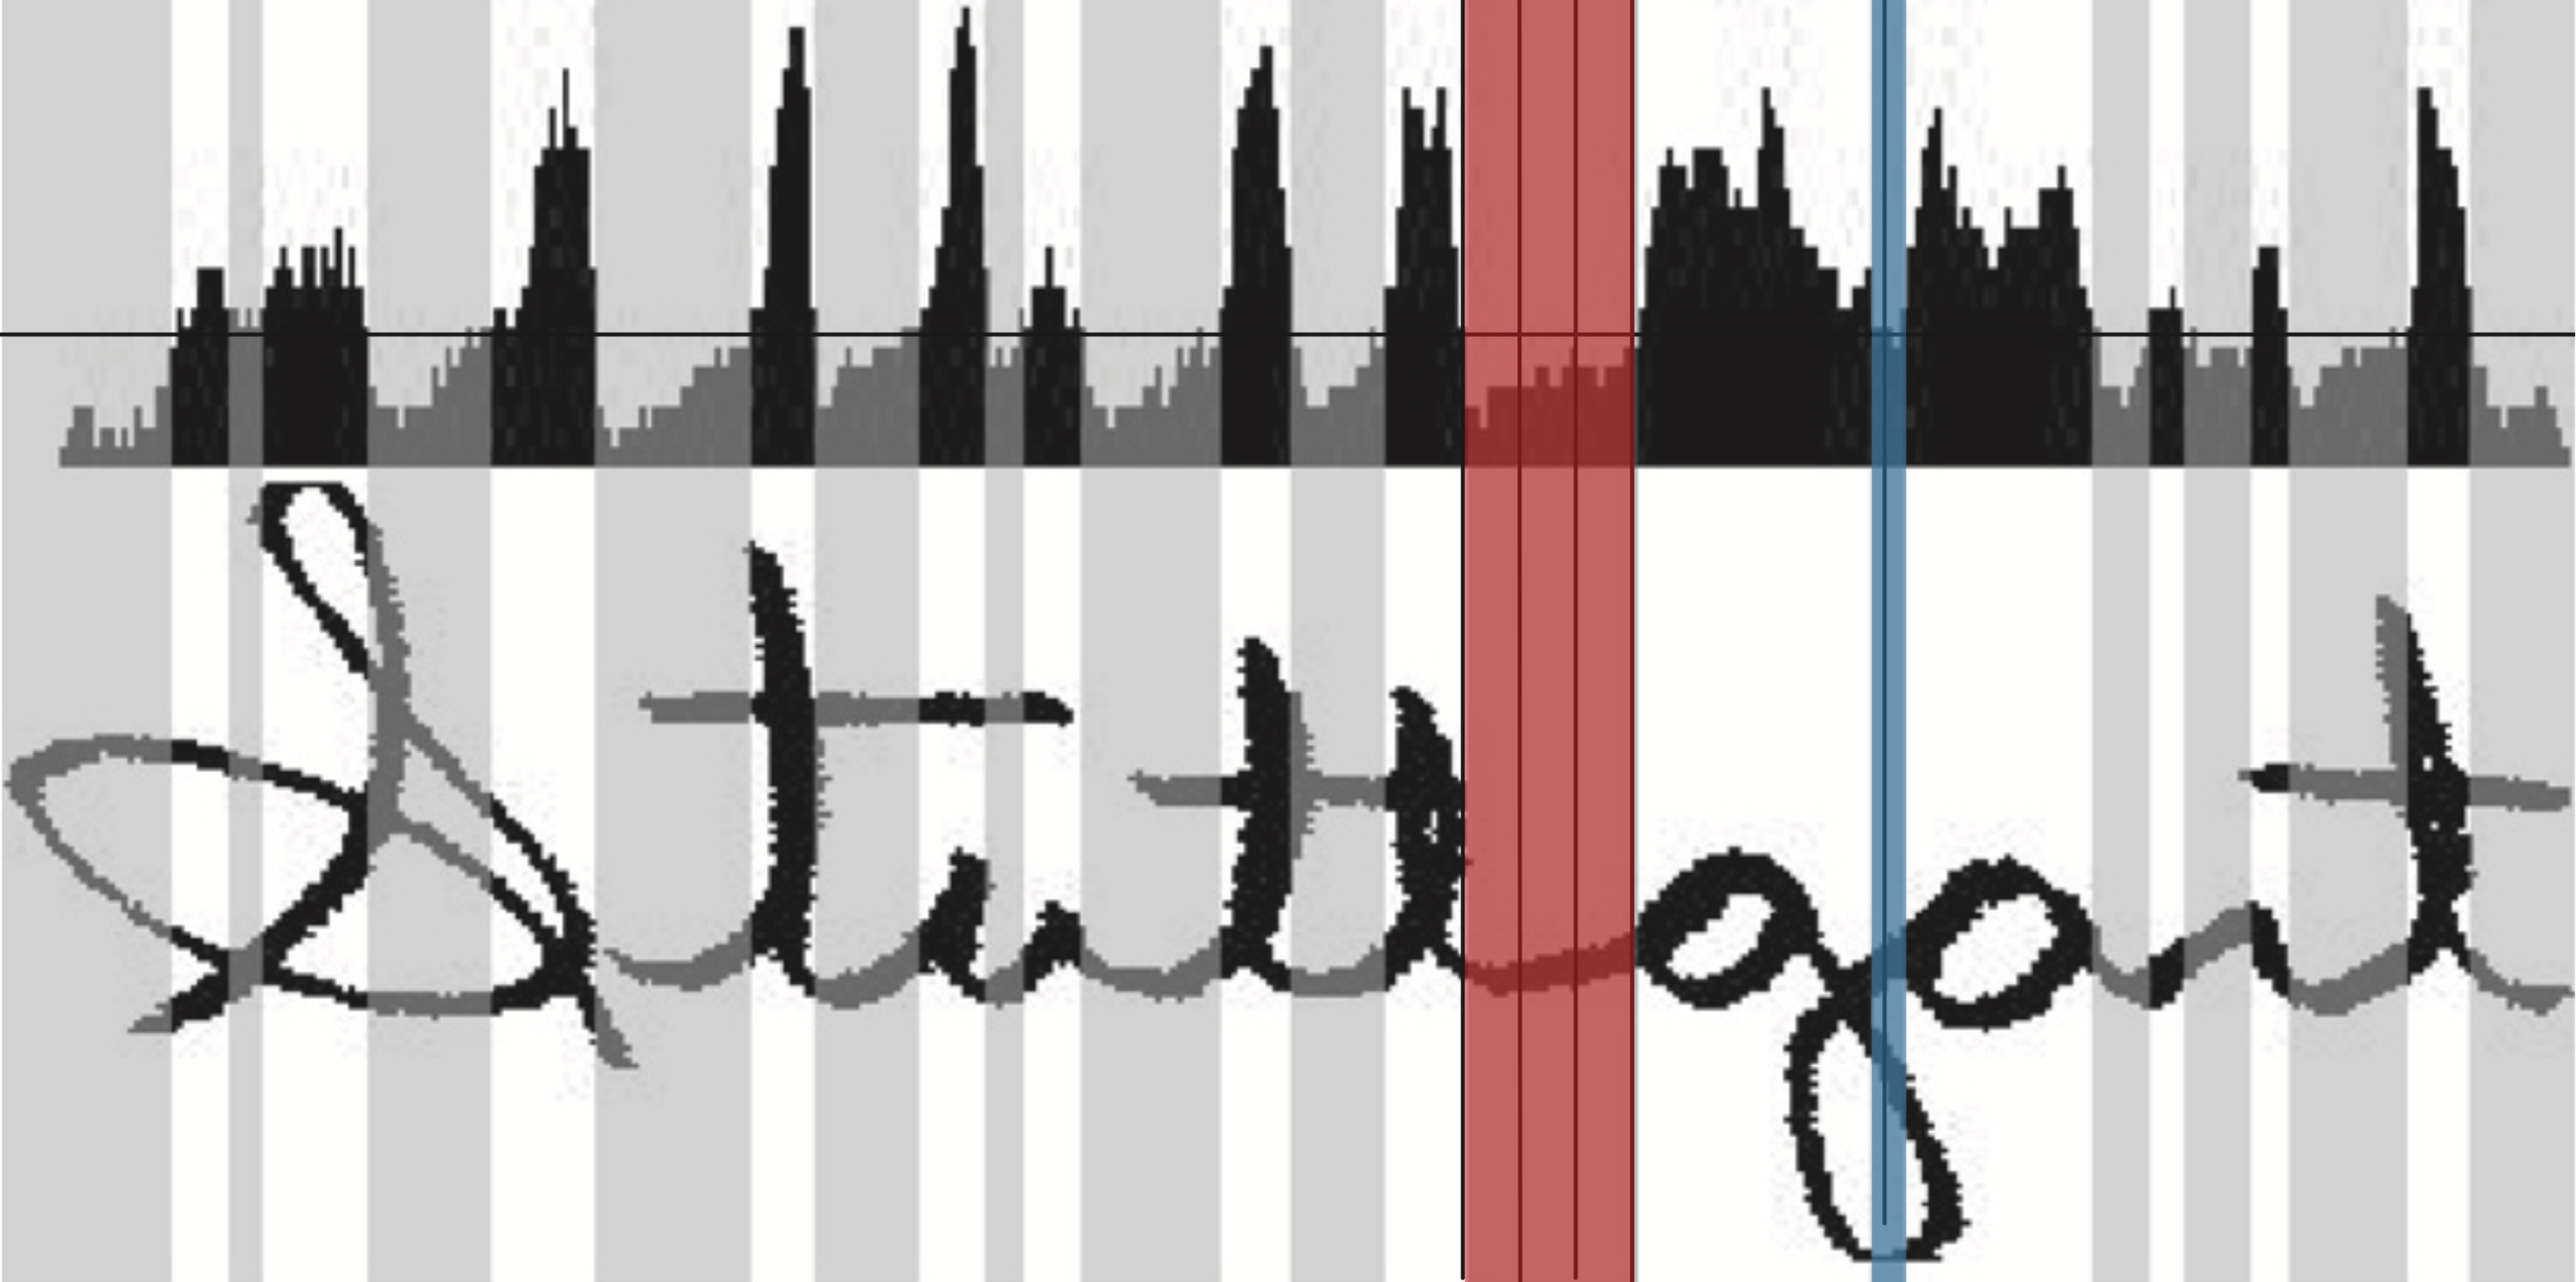
\includegraphics[width=\columnwidth]{shared/img/method/suspicious_regions.png}
		\caption{The vertical pixel density of the body of the image is shown above the word image.  The threshold for suspicious regions is shown as a line in this histogram. The shaded areas show the suspicious regions. For the regions shaded in a color the lines associated with the segmentations points are drawn. The image is adapted from \cite{lee2012binary}.}
		\label{fig:method:segmentation:suspiciousRegions}
	\end{figure}

	The initial set of segmentation points is determined based on these regions. If the width of a region is smaller than the minimum character width a segmentation point is placed in the middle of this region, as illustrated by the blue region in \cref{fig:method:segmentation:suspiciousRegions}. In regions with a width greater than or equal to the minimum character width, such as the red region in \cref{fig:method:segmentation:suspiciousRegions}, segmentation points are placed at the start and the end of the region. Between these boundaries segmentation points are placed with an intervals of minimum character width. These initial segmentation points are filtered before the actual segmentation commences.

	Firstly all segmentation lines that cross a hole, i.e. a region of background pixels completely surrounded by foreground pixels, are removed. Holes are detected via region growing algorithm. 

	After all segmentation lines crossing a hole have been removed we move the segmentation lines in such a way that in the final positioning the distance between two segmentation lines is always greater than the minimum character width. To this end we iterate over all neighboring pairs of segmentation lines from left to right. If the distance between the two lines that make up the pair is smaller than the the minimum character width, the two lines are replaced by one line in the horizontal center of the regions defined by the pair.  This process is recursively repeated recursively for the segmentation lines to the left and to right of the new line. The resulting set of lines is used for the segmentation.

	\begin{figure}[t]
		\centering
		\subfloat[]{
			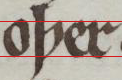
\includegraphics[height=7em]{shared/img/method/base_line_succes.png}%
			\label{fig:method:segmentation:baseline:succes}%
		}
		\hspace{0.05\columnwidth}
		\subfloat[]{
			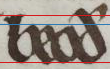
\includegraphics[height=7em]{shared/img/method/base_line_fail.png}%
			\label{fig:method:segmentation:baseline:failure}%
		}
		\caption{An example of \protect\subref{fig:method:segmentation:baseline:succes} correct and \protect\subref{fig:method:segmentation:baseline:failure} incorrect found baselines. The computed baselines are shown in red. If the found baselines were incorrect, the expected baselines are shown in blue.}
		\label{fig:method:segmentation:baseline}
	\end{figure}

\subsubsection{Select Sub-Image}
\label{sss:method:segmentaton:selectsubimage}
	As shown in \cref{alg:method:segmentation:algorithm} the algorithm keeps track of two lists, one with character images, \characters, and one with images that need to be segmented further, \segmentfurther. At the start of each iteration the image with the highest width over height ratio is selected for further segmentation from the second list. This selection criterion assumes that the widest image is the most likely to contain multiple characters. It should be noted that the height of the images is not the same for all images, as white borders are removed from \image,\leftsubimage and \rightsubimage before they are returned from \function{SPLIT}{}. This reduces the influence of sloppy word bounding boxes or segmentation lines on the segmentation.

\subsubsection{Select Segmentation Point}
\label{sss:method:segmentaton:selectssp}
	\segmentationpoint is selected according to two scores: the distance score, $s_{\text{distance}}$ and the vertical pixel density score, $s_{\text{density}}$. The distance score of segmentation $l_x$ in an image with horizontal center $c_x$ is defined as
		\begin{equation}\label{eq:method:segmenation:selectSP:distancecriterion}
			s_{\text{distance}} = \frac{\abs{c_x - l_x}}{c_x}.
		\end{equation}
	This score score promotes the selection of a segmentation line near the center of the image, which should reduce chain failure. The pixel density score promotes the selection of segmentation points at white space that separates two characters. Let the height of the sub image be $w$ and $l_d$ the pixel density underneath the segmentation line $l$, then
		\begin{equation}
			s_{\text{density}} = \frac{l_d}{w}.
		\end{equation}
	Both scores are summed, the line with the lowest score is selected as the segmentation point.

\subsubsection{Split}
\label{sss:method:segmentaton:splitimage}

	The simplest way to split the image along the segmentation line, $l$, is to designate all pixel to the left of the line to \leftsubimage, and all pixels to the right of the line to \rightsubimage. However this can result in artifacts as illustrated in \cref{fig:method:segmentation:splitting:straight}, where part of the `n' is added to the `i', resulting in a letter that looks more like a `c' than an `i' in \leftsubimage.

	\begin{figure}[t]
		\centering
		\subfloat[]{
			\resizebox {0.45\columnwidth} {!} {
				\begin{tikzpicture}
					[
						noname/.style={%
						rectangle,
						text height=1.5ex,
						text depth=.25ex,
						text width=1em,
						text centered,
						minimum height=1em
			  		}]
				    \node[anchor=south west,inner sep=0] (image) at (0,0) {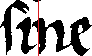
\includegraphics[width=0.45\columnwidth]{shared/img/method/split_straight_path.png}};
				    \begin{scope}[x={(image.south east)},y={(image.north west)}]
				    	\node [anchor=south, noname] (s) at (0.4130434783,1.1) {$s$}; 
				    	\node[draw=none] (saux) at (0.4130434783,0.95) {};
						\draw[->] (s) edge (saux);
						%
				    	\node [anchor=north, noname] (g) at (0.4130434783,-0.1) {$g$}; 
				    	\node[draw=none] (gaux) at (0.4130434783,0.05) {};
						\draw[->] (g) edge (gaux);						
				    \end{scope}
				\end{tikzpicture}
			}			
			\label{fig:method:segmentation:splitting:straight}%			
		}
		\hfill
		\subfloat[]{
			\resizebox {0.45\columnwidth} {!} {
				\begin{tikzpicture}
					[
						noname/.style={%
						rectangle,
						text height=1.5ex,
						text depth=.25ex,
						text width=1em,
						text centered,
						minimum height=1em
			  		}]
				    \node[anchor=south west,inner sep=0] (image) at (0,0) {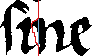
\includegraphics[width=0.45\columnwidth]{shared/img/method/split_astar_path.png}};
				    \begin{scope}[x={(image.south east)},y={(image.north west)}]
				    	\node [anchor=south, noname] (s) at (0.4130434783,1.1) {$s$}; 
				    	\node[draw=none] (saux) at (0.4130434783,0.95) {};
						\draw[->] (s) edge (saux);
						%
				    	\node [anchor=north, noname] (g) at (0.4130434783,-0.1) {$g$}; 
				    	\node[draw=none] (gaux) at (0.4130434783,0.05) {};
						\draw[->] (g) edge (gaux);						
				    \end{scope}
				\end{tikzpicture}
			}			
			\label{fig:method:segmentation:splitting:astar}%			
		}
		\caption{Splitting based on a segmentation point, shown as a blue line, along \protect\subref{fig:method:segmentation:splitting:straight} a straight path and \protect\subref{fig:method:segmentation:splitting:astar} a path found with \astar. The used path are shown in red. The arrows indicate the position of the goal and destination pixels, $s$ and $g$ respectively.}
		\label{fig:method:segmentation:splitting:comparison}
	\end{figure}

	In \cref{fig:method:segmentation:splitting:astar} the image is split along a path that keeps both characters intact. This path is found by looking for a path from $s$ to $g$ with \astar. From some pixel only its four-connected neighbors can be reached. The path is searched in the area defined by a rectangle with minimum character width and image height centered on the segmentation line. The heuristic distance from pixel $n$ to the goal pixel, $g$ is the Manhattan distance between the two pixels:
	\begin{equation}\label{eq:method:segmentation:heuristic}
		h(n) = \abs{g_x - n_x} + \abs{g_y - n_y},
	\end{equation}
	as we are traversing a four connected pixel grid.
	The cost of getting from pixel $s$, to pixel $n$ is defined as:
	\begin{equation}\label{eq:method:segmentation:costFunction}
		g(n) = 
		\begin{cases}
			g(n') + 1	& \text{if } n \text{ is a background pixel.}\\
			g(n') + i 	& \text{if } n \text{ is a foreground pixel on $l$.}\\
			\infty 		& \text{otherwise.}
		\end{cases}
	\end{equation}
	where $i$ is the intersection penalty and $n'$ is the four connected neighbor from which we reached $n$. \Cref{eq:method:segmentation:costFunction} ensurers that the path only intersects foreground pixels if they lie on the segmentation line. Furthermore the intersection penalty ensures that characters are only split along a winding path if a straight path is not possible. We have set the intersection penalty, $i$, to 5. If there are no foreground pixels underneath the segmentation line, the distance function reduces to the Minkowski distance with $p = 1$. 

\subsubsection{Detecting a Character Image}
\label{sss:method:segmentaton:segmentfurther}
	We decide if a sub image is a character or if it should be segmented further based on three properties of the sub image: the width, the height and the number of foreground pixels. The sub image should satisfy two conditions to be considered a character: Its width should be between between the minimum and maximum image width. And the number of foreground pixels should be greater than the minimum number of foreground pixels.

	An image is considered for further segmentation if it satisfies three conditions: it should have segmentation lines, the number of foreground pixels and the image width should be greater than twice the minimum of these values in the train data.

	If neither of the preceding sets of conditions are satisfied the image is considered for further segmentation if its width is greater than the mean character width and it has segmentation lines. If its width is less than two standard deviations away from the mean character width it is added to \characters, otherwise it is discarded.

\subsubsection{Continue}
\label{sss:method:segmentaton:termination}
	Segmentation is continued as long as the following conditions are satisfied: we have not yet found more characters than the length of the longest word in the lexicon and there are still images in the list \segmentfurther. 

\subsection{Feature Extraction}
\label{ss:methods:featureExtraction}
%!TEX root = ../../main.tex
While we considered using various features for the character recognition such as crossing, projection histograms and celled projections \cite{HWR:features1}\cite{HWR:features2}. From all the above the celled projections report the best results (7\% and 10\% better than crossings and projections respectively) \cite{HWR:features1}.

Celled projections are extracted as follows. First the area of the character is split into regions, vertically, horizontally or mixed. In \ref{fig:method:features:feature} we see an example of vertical projection. Then for each of the regions we acquire the projections of the pixels on the left border of the region. This way binary vectors are created which then we concatenate.

\begin{figure}[t!]
	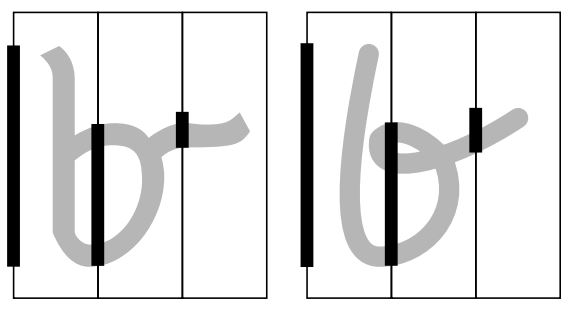
\includegraphics[width=8cm]{shared/img/projection_letter.jpg}
	\caption{In the above picture we see that even if the characters are differently written the projection feature will still extract consistent vectors.}
	\label{fig:method:features:feature}
\end{figure}

\subsection{Recognition}
\label{ss:methods:recognition}
%!TEX root = ../../main.tex
\laura{Which value for $k$}
\laura{Which distance measure}
\laura{Which optimization for KNN}


As stated before we have chosen to focus most of the efforts of our classifier on the earlier stages in the process. Consequently we have opted for a simple classifier, that performs well on handwriting\cite{lee1991handwritten,smith1994handwritten,ha1997off}, namely the $k$-nearest neighbor algorithm. This classifier assigns to a new pattern the most frequent class of its $k$ nearest neighbors according to some distance measure. 

We have chosen $k = \sqrt{n}$ where $n$ is the number of neighbors of the unclassified pattern \cite{duda2012pattern}. As a distance measure we use the Minkowski similarity measure with $p = 2$ to determine the distance between two patterns.

\subsection{Post Processing}
\label{ss:methods:postprocessing}
%!TEX root = ../../main.tex
\todo[inline]{How do we do post processing}
\todo[inline]{How are priors computed}
\todo[inline]{Which distance measure is used}

\section{Results}
\label{s:results}
%!TEX root = ../main.tex
\begin{table*}[t]
\caption{LOOCV Error}
\label{tab:results:loocv}
\centering
	\begin{tabular}{lcccccccc}
		\toprule
					& \multicolumn{4}{c}{Validation} & \multicolumn{4}{c}{Binary}\\
					\cmidrule(r){2-5} \cmidrule(r){6-9}
		~ 			& $\mu$ 	& $\sigma$ 	& min 	& max 	& $\mu$ 	& $\sigma$ 	& min 	& max \\
		\midrule
		All 		& 0.694 	& 0.165 	& 0.3 	& 1.0 	& 0.718 	& 0.133 	& 0.25 	& 1.0 \\
		Bohemians 	& 0.731 	& 0.131 	& 0.44 	& 0.982 & 0.737 	& 0.11 		& 0.5 	& 0.982 \\
		Homilies 	& 0.647 	& 0.194 	& 0.214 & 1.0 	& 0.686 	& 0.171 	& 0.25 	& 1.0 \\
		\bottomrule
	\end{tabular}
\end{table*}
%
To measure how well the binary over segmentation performed we have compared this algorithm with a base line, `validation segmentation'. This baseline uses the character boundaries provided by the annotation files in the training data. When computing the error we only considered words of which the internal segmentation was complete in the annotation file. We have defined the error of one file as the number of incorrectly classified words divided by the number of completely internally segmented words in the annotation file. \Cref{tab:results:loocv} presents the results of LOOCV with (subsets) of the train data. 

We observe that the validation segmentation gets better results than the binary over segmentation. Furthermore independent of the segmentation algorithm the recognizer performs better on the pages from ``Chronicles of the Bohemians" than on pages from ``Old English Homilies".

Testing the results on previously unseen test data we find that the recognition rate for ``Chronicles of the Bohemians" is 2.28\%, for ``Old English Homilies" it is $3.88\%$ and on both books combined it is $2.56\%$ \footnote{It should be noted that these results were gathered using an earlier version of the classifier that did not move segmentation points based on the width between neighboring segmentation points.}

\section{Discussion}
\label{s:discussion}
%!TEX root = /Users/laura/Repositories/HandwritingRecognition/report/main.tex
The results presented in the previous section show that our recognizer did not perform very well. The sections below discuss of several of the components what might have affected their performance and how it could be improved.

\subsection{Preprocessing}
\label{ss:discussion:preprocessing}
%!TEX root = ../../main.tex
For the handwriting to be effective we had to bring the data into a clean state. To this end we used a pipeline which is described below in figure \ref{fig:pipeline}. 

\begin{figure}[ht]
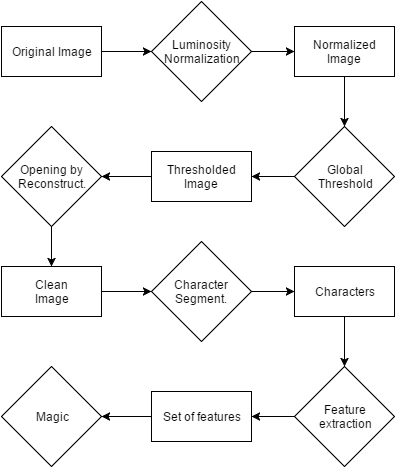
\includegraphics[width=8cm]{shared/img/pipeline.png}
\caption{Overview of our pipeline.}
\label{fig:pipeline}
\end{figure}

As the figure explains the first step is to normalize the luminosity of the image. This step is essential for the thresholding to work since in some parts of dataset the ink has worn off the pages. \Cref{fig:methods:preprocessing:lumNormalization} gives an example why luminosity normalization was necessary. In the above mentioned figure, we applied the same threshold filter with and without luminosity normalization and the results speak for themselves. By normalizing the luminosity we eliminate the need to adjust threshold values in later steps.

\begin{figure}
	\centering
	\subfloat[]{
		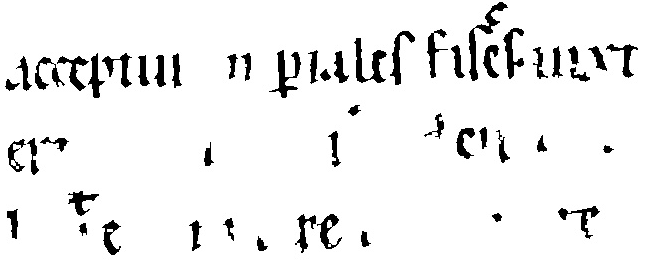
\includegraphics[width=\columnwidth]{shared/img/before_lum.png}%
		\label{fig:methods:preprocessing:lumNormalization:before}%
	}
	\hfil
	\subfloat[]{
		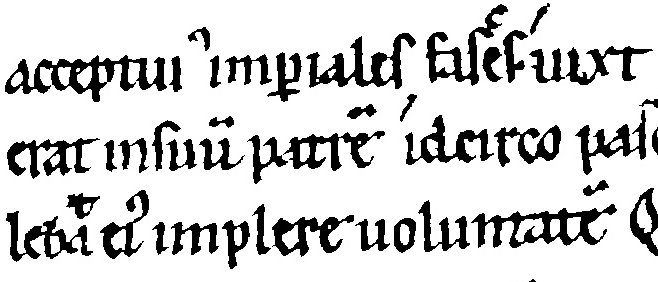
\includegraphics[width=\columnwidth]{shared/img/after_lum.png}%
		\label{fig:methods:preprocessing:lumNormalization:after}%
	}
	\caption{An image of text \protect\subref{fig:methods:preprocessing:lumNormalization:before} before and \protect\subref{fig:methods:preprocessing:lumNormalization:after} after luminization normalization.}
	\label{fig:methods:preprocessing:lumNormalization}
\end{figure}

The next step is to binarize the image and extract the clean text from it. For the binarization we tested the Otsu approach and global threshold and we settled with the first as it gave better results. To eliminate the what is left from the noise we applied opening by reconstruction. This has a result to miss some punctuation characters which however did not prove crucial to our learning process. %In figure \ref{} we can see the final result of the preprocessing of the data. 

\subsection{Internal Segmentation}
\label{ss:discussion:characterSegmentation}
%!TEX root = ../../main.tex
\newcommand{\body}{\ensuremath{\t{body}}\xspace}
\newcommand{\strokewidth}{\ensuremath{\t{stroke\_w}}\xspace}
\newcommand{\segmentationpoints}{\ensuremath{\t{sps}}\xspace}
\newcommand{\segmentationpoint}{\ensuremath{\t{sp}}\xspace}
\newcommand{\image}{\ensuremath{\t{image}}\xspace}
\newcommand{\subimage}{\ensuremath{\t{sub\_image}}\xspace}
\newcommand{\leftsubimage}{\ensuremath{\t{left}}\xspace}
\newcommand{\rightsubimage}{\ensuremath{\t{right}}\xspace}
\newcommand{\segmentfurther}{\ensuremath{\t{todo}}\xspace}
\newcommand{\characters}{\ensuremath{\t{done}}\xspace}
\newcommand{\parameters}{\ensuremath{\t{parameters}}\xspace}

\begin{figure}[t]
	%!TEX root = ../../main.tex
\MakeRobust{\Call}

\begin{algorithmic}[0]
\Function{segment}{$\image,\, \parameters$}
\label{alg:line:bodyregion} \State \body $\gets$ \Call{body\_region}{\image}
\label{alg:line:strokewidth} \State \strokewidth $\gets$ \Call{stroke\_width}{\image} 
\item[]
\label{alg:line:segmentationpoints} \State \segmentationpoints $\gets$ \Call{segmentation\_points}{\body, \strokewidth} 
\State \segmentfurther, \characters $\gets$ [\image], []
\item[]
\label{alg:line:whileCondition} \While{\Call{continue}{~}}
	\label{alg:line:selectSubImage}\State $\subimage \gets$ \Call{select\_sub\_image}{\segmentfurther} 
	\label{alg:line:selectSegmentationPoint}\State $\segmentationpoint \gets$ \Call{select\_sp}{\segmentationpoints} 
	\label{alg:line:split}\State \leftsubimage, \rightsubimage $\gets$ \Call{split}{\subimage, \segmentationpoint}
	%
	\State \Call{add\_to\_correct\_list}{\leftsubimage, \characters, \segmentfurther}
	\State \Call{add\_to\_correct\_list}{\rightsubimage, \characters, \segmentfurther}
\EndWhile
\label{alg:line:merge}\State \textbf{return} \Call{merge}{\segmentfurther, \characters}
\EndFunction
\end{algorithmic}
	\caption{The Binary Over Segmentation Algorithm.}
	\label{alg:method:segmentation:algorithm}
\end{figure}

We use a form of binary over segmentation to recognize characters in the word, see \cref{alg:method:segmentation:algorithm}. This algorithm aims to segment an image on the most likely segmentation point. If these sub images are not characters they can be selected again for further segmentation. This segmenting of sub images is repeated until the termination condition has been reached. The final list of characters is the list of characters, \characters, merged with the list of images that could be segmented further, \segmentfurther. This merge also ensures that the order of the images is correct.

The \parameters passed to \function{segment}{} in \cref{alg:method:segmentation:algorithm} contain the maximum word length and the minimum, mean and maximum image width, height and number of foreground pixels. Other than maximum word length, these parameters are computed based on the train data, by collecting these data from each character image, the minimum, mean and maximum are computed over all measurements that fall within two standard deviations of the mean. The maximum word length is simply the length of the longest word in the train data.

The different functions used in \cref{alg:method:segmentation:algorithm} are discussed in \crefrange{sss:method:segmentaton:bodyregion}{sss:method:segmentaton:termination}.

\subsubsection{Body Region}
\label{sss:method:segmentaton:bodyregion}
	The body region is the part of the image between the lower and upper base line. The lower base line is computed as the mode of the minimum row index with a foreground pixel in each column. The upper baseline is computed similarly, but uses the maximum row index.

	Using the body region for the computation of the segmentation points reduces the influence of extensive ligatures \cite{lee2012binary}. \Cref{fig:method:segmentation:baseline} presents some examples of computed baselines. The first example, \Cref{fig:method:segmentation:baseline:succes}, reflects the intended outcome. The second example, \cref{fig:method:segmentation:baseline:failure}, draws the upper baseline too high, probably due too the extra curve on the last letter.

\subsubsection{Stroke Width}
\label{sss:method:segmentaton:strokwidth}
	The stroke width refers to how thick the stroke of a pen is. It is computed as the mode of the number of sequential foreground pixels in one row or column of pixels. As different pens or authors can write on the same page it is more robust to compute the stroke width per word image instead of per page image.

\subsubsection{Segmentation Points}
\label{sss:method:segmentaton:segmentationpoints}
	To find the segmentation lines we first determine the suspicious regions. A suspicious region is a region in the body of the word image where the vertical pixel density is greater than some threshold, $2 \cdot \strokewidth$. \Cref{fig:method:segmentation:suspiciousRegions} illustrates the suspicious regions found in a word. 

	\begin{figure}
		\centering
		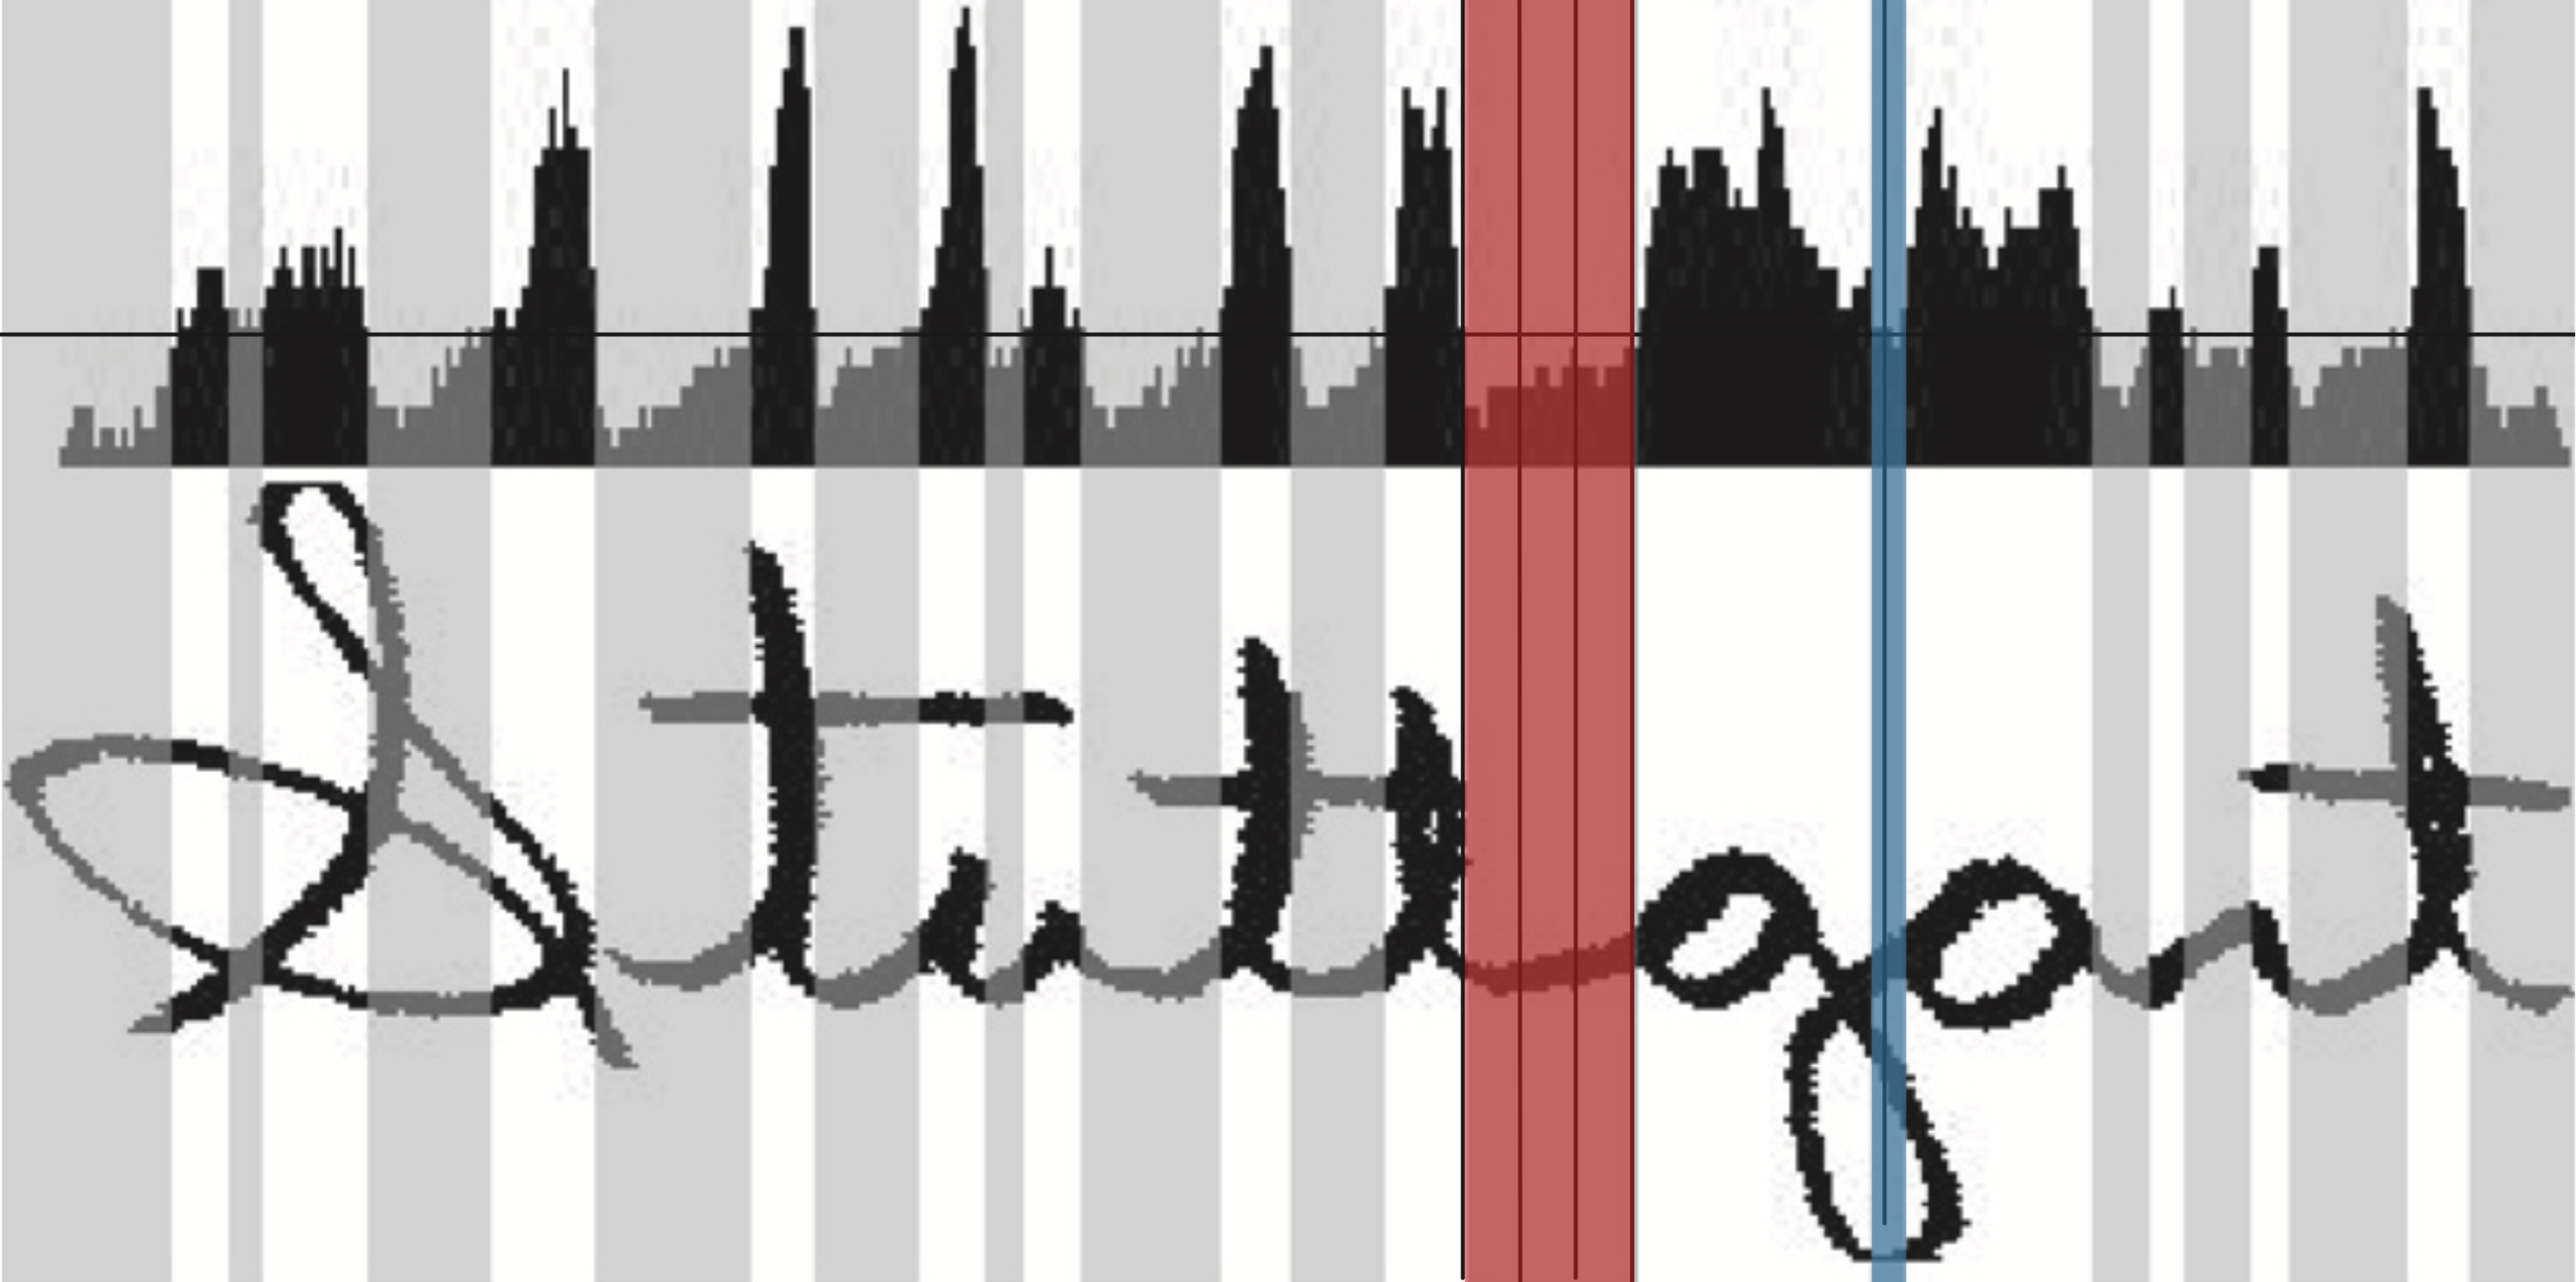
\includegraphics[width=\columnwidth]{shared/img/method/suspicious_regions.png}
		\caption{The vertical pixel density of the body of the image is shown above the word image.  The threshold for suspicious regions is shown as a line in this histogram. The shaded areas show the suspicious regions. For the regions shaded in a color the lines associated with the segmentations points are drawn. The image is adapted from \cite{lee2012binary}.}
		\label{fig:method:segmentation:suspiciousRegions}
	\end{figure}

	The initial set of segmentation points is determined based on these regions. If the width of a region is smaller than the minimum character width a segmentation point is placed in the middle of this region, as illustrated by the blue region in \cref{fig:method:segmentation:suspiciousRegions}. In regions with a width greater than or equal to the minimum character width, such as the red region in \cref{fig:method:segmentation:suspiciousRegions}, segmentation points are placed at the start and the end of the region. Between these boundaries segmentation points are placed with an intervals of minimum character width. These initial segmentation points are filtered before the actual segmentation commences.

	Firstly all segmentation lines that cross a hole, i.e. a region of background pixels completely surrounded by foreground pixels, are removed. Holes are detected via region growing algorithm. 

	After all segmentation lines crossing a hole have been removed we move the segmentation lines in such a way that in the final positioning the distance between two segmentation lines is always greater than the minimum character width. To this end we iterate over all neighboring pairs of segmentation lines from left to right. If the distance between the two lines that make up the pair is smaller than the the minimum character width, the two lines are replaced by one line in the horizontal center of the regions defined by the pair.  This process is recursively repeated recursively for the segmentation lines to the left and to right of the new line. The resulting set of lines is used for the segmentation.

	\begin{figure}[t]
		\centering
		\subfloat[]{
			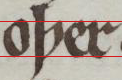
\includegraphics[height=7em]{shared/img/method/base_line_succes.png}%
			\label{fig:method:segmentation:baseline:succes}%
		}
		\hspace{0.05\columnwidth}
		\subfloat[]{
			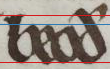
\includegraphics[height=7em]{shared/img/method/base_line_fail.png}%
			\label{fig:method:segmentation:baseline:failure}%
		}
		\caption{An example of \protect\subref{fig:method:segmentation:baseline:succes} correct and \protect\subref{fig:method:segmentation:baseline:failure} incorrect found baselines. The computed baselines are shown in red. If the found baselines were incorrect, the expected baselines are shown in blue.}
		\label{fig:method:segmentation:baseline}
	\end{figure}

\subsubsection{Select Sub-Image}
\label{sss:method:segmentaton:selectsubimage}
	As shown in \cref{alg:method:segmentation:algorithm} the algorithm keeps track of two lists, one with character images, \characters, and one with images that need to be segmented further, \segmentfurther. At the start of each iteration the image with the highest width over height ratio is selected for further segmentation from the second list. This selection criterion assumes that the widest image is the most likely to contain multiple characters. It should be noted that the height of the images is not the same for all images, as white borders are removed from \image,\leftsubimage and \rightsubimage before they are returned from \function{SPLIT}{}. This reduces the influence of sloppy word bounding boxes or segmentation lines on the segmentation.

\subsubsection{Select Segmentation Point}
\label{sss:method:segmentaton:selectssp}
	\segmentationpoint is selected according to two scores: the distance score, $s_{\text{distance}}$ and the vertical pixel density score, $s_{\text{density}}$. The distance score of segmentation $l_x$ in an image with horizontal center $c_x$ is defined as
		\begin{equation}\label{eq:method:segmenation:selectSP:distancecriterion}
			s_{\text{distance}} = \frac{\abs{c_x - l_x}}{c_x}.
		\end{equation}
	This score score promotes the selection of a segmentation line near the center of the image, which should reduce chain failure. The pixel density score promotes the selection of segmentation points at white space that separates two characters. Let the height of the sub image be $w$ and $l_d$ the pixel density underneath the segmentation line $l$, then
		\begin{equation}
			s_{\text{density}} = \frac{l_d}{w}.
		\end{equation}
	Both scores are summed, the line with the lowest score is selected as the segmentation point.

\subsubsection{Split}
\label{sss:method:segmentaton:splitimage}

	The simplest way to split the image along the segmentation line, $l$, is to designate all pixel to the left of the line to \leftsubimage, and all pixels to the right of the line to \rightsubimage. However this can result in artifacts as illustrated in \cref{fig:method:segmentation:splitting:straight}, where part of the `n' is added to the `i', resulting in a letter that looks more like a `c' than an `i' in \leftsubimage.

	\begin{figure}[t]
		\centering
		\subfloat[]{
			\resizebox {0.45\columnwidth} {!} {
				\begin{tikzpicture}
					[
						noname/.style={%
						rectangle,
						text height=1.5ex,
						text depth=.25ex,
						text width=1em,
						text centered,
						minimum height=1em
			  		}]
				    \node[anchor=south west,inner sep=0] (image) at (0,0) {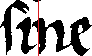
\includegraphics[width=0.45\columnwidth]{shared/img/method/split_straight_path.png}};
				    \begin{scope}[x={(image.south east)},y={(image.north west)}]
				    	\node [anchor=south, noname] (s) at (0.4130434783,1.1) {$s$}; 
				    	\node[draw=none] (saux) at (0.4130434783,0.95) {};
						\draw[->] (s) edge (saux);
						%
				    	\node [anchor=north, noname] (g) at (0.4130434783,-0.1) {$g$}; 
				    	\node[draw=none] (gaux) at (0.4130434783,0.05) {};
						\draw[->] (g) edge (gaux);						
				    \end{scope}
				\end{tikzpicture}
			}			
			\label{fig:method:segmentation:splitting:straight}%			
		}
		\hfill
		\subfloat[]{
			\resizebox {0.45\columnwidth} {!} {
				\begin{tikzpicture}
					[
						noname/.style={%
						rectangle,
						text height=1.5ex,
						text depth=.25ex,
						text width=1em,
						text centered,
						minimum height=1em
			  		}]
				    \node[anchor=south west,inner sep=0] (image) at (0,0) {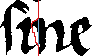
\includegraphics[width=0.45\columnwidth]{shared/img/method/split_astar_path.png}};
				    \begin{scope}[x={(image.south east)},y={(image.north west)}]
				    	\node [anchor=south, noname] (s) at (0.4130434783,1.1) {$s$}; 
				    	\node[draw=none] (saux) at (0.4130434783,0.95) {};
						\draw[->] (s) edge (saux);
						%
				    	\node [anchor=north, noname] (g) at (0.4130434783,-0.1) {$g$}; 
				    	\node[draw=none] (gaux) at (0.4130434783,0.05) {};
						\draw[->] (g) edge (gaux);						
				    \end{scope}
				\end{tikzpicture}
			}			
			\label{fig:method:segmentation:splitting:astar}%			
		}
		\caption{Splitting based on a segmentation point, shown as a blue line, along \protect\subref{fig:method:segmentation:splitting:straight} a straight path and \protect\subref{fig:method:segmentation:splitting:astar} a path found with \astar. The used path are shown in red. The arrows indicate the position of the goal and destination pixels, $s$ and $g$ respectively.}
		\label{fig:method:segmentation:splitting:comparison}
	\end{figure}

	In \cref{fig:method:segmentation:splitting:astar} the image is split along a path that keeps both characters intact. This path is found by looking for a path from $s$ to $g$ with \astar. From some pixel only its four-connected neighbors can be reached. The path is searched in the area defined by a rectangle with minimum character width and image height centered on the segmentation line. The heuristic distance from pixel $n$ to the goal pixel, $g$ is the Manhattan distance between the two pixels:
	\begin{equation}\label{eq:method:segmentation:heuristic}
		h(n) = \abs{g_x - n_x} + \abs{g_y - n_y},
	\end{equation}
	as we are traversing a four connected pixel grid.
	The cost of getting from pixel $s$, to pixel $n$ is defined as:
	\begin{equation}\label{eq:method:segmentation:costFunction}
		g(n) = 
		\begin{cases}
			g(n') + 1	& \text{if } n \text{ is a background pixel.}\\
			g(n') + i 	& \text{if } n \text{ is a foreground pixel on $l$.}\\
			\infty 		& \text{otherwise.}
		\end{cases}
	\end{equation}
	where $i$ is the intersection penalty and $n'$ is the four connected neighbor from which we reached $n$. \Cref{eq:method:segmentation:costFunction} ensurers that the path only intersects foreground pixels if they lie on the segmentation line. Furthermore the intersection penalty ensures that characters are only split along a winding path if a straight path is not possible. We have set the intersection penalty, $i$, to 5. If there are no foreground pixels underneath the segmentation line, the distance function reduces to the Minkowski distance with $p = 1$. 

\subsubsection{Detecting a Character Image}
\label{sss:method:segmentaton:segmentfurther}
	We decide if a sub image is a character or if it should be segmented further based on three properties of the sub image: the width, the height and the number of foreground pixels. The sub image should satisfy two conditions to be considered a character: Its width should be between between the minimum and maximum image width. And the number of foreground pixels should be greater than the minimum number of foreground pixels.

	An image is considered for further segmentation if it satisfies three conditions: it should have segmentation lines, the number of foreground pixels and the image width should be greater than twice the minimum of these values in the train data.

	If neither of the preceding sets of conditions are satisfied the image is considered for further segmentation if its width is greater than the mean character width and it has segmentation lines. If its width is less than two standard deviations away from the mean character width it is added to \characters, otherwise it is discarded.

\subsubsection{Continue}
\label{sss:method:segmentaton:termination}
	Segmentation is continued as long as the following conditions are satisfied: we have not yet found more characters than the length of the longest word in the lexicon and there are still images in the list \segmentfurther. 

\subsection{Feature Extraction}
\label{ss:discussion:featureExtraction}
%!TEX root = ../../main.tex
While we considered using various features for the character recognition such as crossing, projection histograms and celled projections \cite{HWR:features1}\cite{HWR:features2}. From all the above the celled projections report the best results (7\% and 10\% better than crossings and projections respectively) \cite{HWR:features1}.

Celled projections are extracted as follows. First the area of the character is split into regions, vertically, horizontally or mixed. In \ref{fig:method:features:feature} we see an example of vertical projection. Then for each of the regions we acquire the projections of the pixels on the left border of the region. This way binary vectors are created which then we concatenate.

\begin{figure}[t!]
	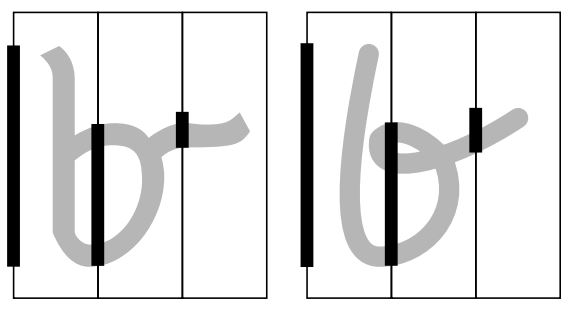
\includegraphics[width=8cm]{shared/img/projection_letter.jpg}
	\caption{In the above picture we see that even if the characters are differently written the projection feature will still extract consistent vectors.}
	\label{fig:method:features:feature}
\end{figure}


\section{Conclusion}
\label{s:conclusion}
%!TEX root = ../main.tex

\bibliographystyle{IEEEtran}
\bibliography{biblio}

%!TEX root = ../main.tex
\begin{IEEEbiographynophoto}{L.E.N. Baakman}
\laura{Contribution to implementation}
\laura{Contribution to paper}
\end{IEEEbiographynophoto}

\begin{IEEEbiographynophoto}{E. Karountzos}
\angelo{Contribution to implementation}
\angelo{Contribution to paper}
\end{IEEEbiographynophoto}

\end{document}


